%%%%%%%%%%%%%%%%%%%%%%%%%%%%%%%%%%%%%%%%%%%%%%%%%%%%%%%%%%%%%%%%%
% Contents: The first start chapter
% $Id: grisbi-manuel-start.tex, v 0.4 2002/10/27 Daniel Cartron
% $Id: grisbi-manuel-start.tex, v 0.5.0 2004/06/01 Loic Breilloux
% $Id: grisbi-manuel-start.tex, v 0.6.0 2011/11/17 Jean-Luc Duflot
% $Id: grisbi-manuel-start.tex, v 0.8.9 2012/04/27 Jean-Luc Duflot
% $Id: grisbi-manuel-start.tex, v 1.0 2014/02/12 Jean-Luc Duflot
%%%%%%%%%%%%%%%%%%%%%%%%%%%%%%%%%%%%%%%%%%%%%%%%%%%%%%%%%%%%%%%%%


\chapter{Initial set-up of Grisbi\label{start}}


\section{Initial Set-up Wizard\label{start-first}}


After installing Grisbi, the first time the software is launched, it will help you with three consecutive wizards:

\begin{enumerate}
	\item The first wizard \enquote{Welcome to Grisbi!}, which will only appear once, on first launch, helps you configure the application. It comprises two steps, the second of which concerns management of the \indexword{account file}\index{account file} (automatic loading and saving, encryption and backup copies).

\begin{figure}[htbp]
	\begin{center}
		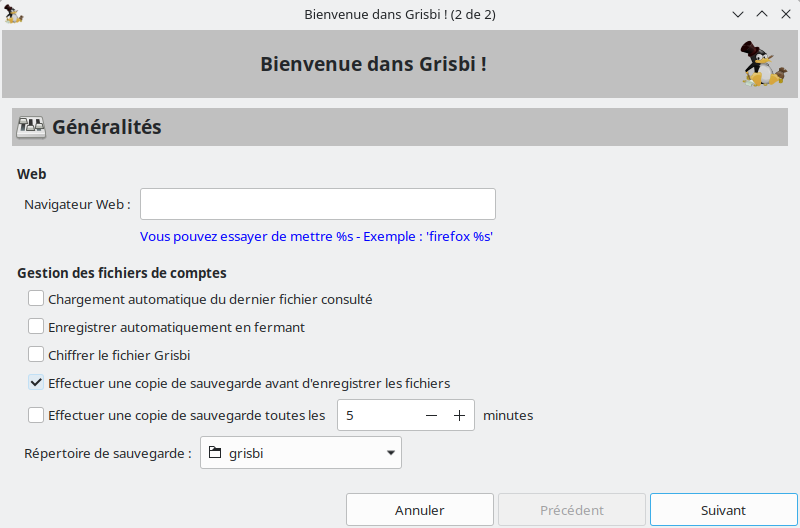
\includegraphics[width=0.98\textwidth]{image/screenshot/start_first_launch}
	\end{center}
	\caption{Initial configuration of accounts file.}
	\label{start_first_launch}
\end{figure}

It is advisable to check the options:
	\begin{itemize}
		\item Automatically load last file on startup%chargement automatique du dernier fichier consulté;
		\item Automatically save on exit;%enregistrer automatiquement en fermant;
		\item Make a backup copy before saving files (checked by default).%effectuer une copie de sauvegarde avant d'enregistrer les fichiers (coché par défaut).
	\end{itemize}
\end{enumerate}

\minisec{\textcolor{red}{\strong{Warning:}}}
The Grisbi developers recommend that you do not use the \menu{Encrypt Grisbi file} option for the following reasons:
\begin{itemize}
	\item there is no method for recovering an encrypted file whose password has been lost;
	\item For some unknown reason, using this option on Windows can render the accounts file completely unusable.
\end{itemize}  
However, if you use it, it is advisable to make regular back-ups of the unencrypted file.

\begin{enumerate}[resume]
	\item The second wizard, \enquote{Welcome to Grisbi!} (or later \enquote{New file Assistant}), which automatically follows the first, includes six steps to help you create the \indexword{account file}\index{account file}.%Le deuxième assistant \frquote{Bienvenue dans Grisbi !} (ou plus tard \frquote{Aide à la création d'un nouveau fichier de comptes}), qui suit automatiquement le premier, comprend six étapes qui vous aiderons à la création du \indexword{fichier de comptes}\index{fichier de comptes}.
	\item This is followed automatically by the third wizard, \enquote{Create a new account}, which is used to create the first account and is described in detail in section \ref{start-newfile} below.%Puis vient automatiquement le troisième assistant \frquote{Créer un nouveau compte} qui permet de créer le premier compte et qui est décrit en détail dans la section \ref{start-newfile} ci-dessous.
\end{enumerate}

At any time you can exit any wizard with the \menu{Cancel} button.

If you do not want to use the Set-up Wizard, you can open a example file instead (see the next section \ref{start-example} below).



\section{Example file\label{start-example}}


If you want to use Grisbi immediately without having to go through the full set-up, for example to get an idea of the possibilities of this program, you can download the  \file{Example\_3.0-en.gsb} file from \lang{Sourceforge.net}\footnote{\urlSourceForgeDocumentation{}} website in the folder \enquote{textsf{examples}}.

% espace avant Attention ou Note :  mm
\vspacepdf{5mm}
\textbf{Note}: in this example file, the names of the payees etc are pure invention; any similarity with a real person or business is entirely accidental.

\section{Creation of a new accounts file\label{start-newfile}}


The first time you use Grisbi, you will need to create a first
\indexword{accounts file}\index{accounts file}. The \gls{extension} of this file will be \file{.gsb} and its name will be \file{your-file-name.gsb}.

Immediately afterwards, you will need to create at least one account (bank, cash, liability or asset account, described in the chapter \vref{accounts} \menu{Account management}), and then a few other accounts (current, savings, credit, possibly a cash account and a few transition accounts) which will contain their respective transactions.

If you are managing a family, you will normally only have one accounts file, as this allows all the exchanges between your different accounts. If you are managing an association, or another family with no accounting relationship with the first, you will create another accounts file, which will have a different name \file{your-second-file-name.gsb}. This will keep the \indexword{accounting entities}\index{accounting entity} separate.

In other words, all your household accounts are recorded in one accounts file, and all your association accounts are recorded in another accounts file.

% TODO update below

% espace pour changement de thme
\vspacepdf{5mm}

The general procedure for creating an account file is as follows: click on the menu File - New Account File; the account file creation wizard opens, which includes six steps. In the sixth step, the assistant offers you:

\begin{itemize}
\item  create a new account, and then follow the account creation wizard, which itself includes five steps, to create the first account (because it is essential to have at least one account);
\item or to use pre existing data, then use the import wizard, which also includes five steps, to import existing account operations.
\end{itemize}

After creating this first account or importing existing account transactions, if you want to create other accounts, you will return to the end of the process of creating the account file, which will return you in both cases to the create a new account option.


% espace pour changement de thme
\vspacepdf{5mm}
To create your accounts file, click the File - New Account File menu; the detailed procedure is as follows:
enumerate
welcome window: confirm with the Forward button;

To create your accounts file, click the \menu{File - New Account File} menu: the detailed procedure is as follows:

\begin{enumerate}
\item New file assistant welcome window: confirm with the \menu{Forward} button:
\item General configuration
générale\refimage{start-file-create-img}:




\begin{figure}[htbp]
\begin{center}
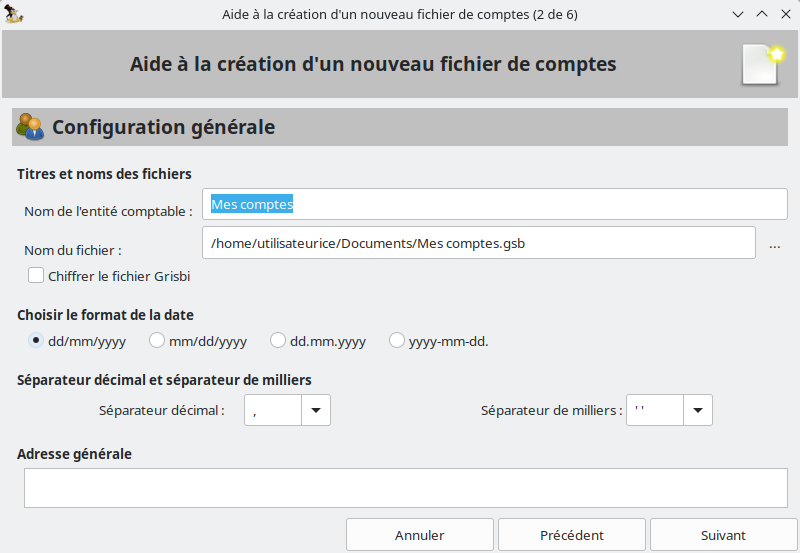
\includegraphics[scale=0.5]{image/screenshot/start_file_create}
\end{center}
\caption{General configuration of an account file}
\label{start-file-create-img}
\end{figure}



\begin{enumerate} 
 \item choose the name of the accounting entity whose accounts you are managing, for example \enquote{My accounts}, which can be chosen as the title of the Grisbi application home page,
\item enter the name of the accounts file with its complete tree; Grisbi defaults to the same name as the reporting entity, but you can change it
\item check the  \menu{Encrypt Grisbi} box if you wish \gls{to encrypt} the accounts file,
\item select the \indexword{date format}\index{date format} with one of the two buttons: dd/mm/yyyy for day/month/year, or  mm/dd/yyyy for month/day/year,
\item choose the decimal \indexword{separator}\index{separator} and the thousands from the drop-down lists,
 \item fill in the address (optional),
 \item  confirm with the  \menu{Forward} button;
\end{enumerate}

\item selection of the base \indexword{currency}\index{currency}:
\begin{enumerate} 
 \item click on the chosen currency in the list,
\item check the "include obsolete currencies" box if you also want to display old currencies,
\item confirm with the \menu{Forward} button;
\end{enumerate}

\item selection of the  \indexword{list of categories}\index{catgories !types} you will use:
\begin{enumerate} 
 \item click on your desired category, either the \menu{Standard category list} or the \menu{Empty list} \footnote{\strong{Translators Note:} Users installing the program on a system with a French Language interface will find different categories are offered including some for business users} 
\item check the \menu{Display foreign category sets} box to check if other categories are available\footnote{\strong{Translators Note:} This option is mainly for the benefit of users of a computer system with the French Language interface who will then be shown the two English categories mentioned in the previous step}
\item confirm with the \menu{Forward} button;
\end{enumerate}

\item Enter details of \indexword{banks}\index{banques !définition} holding your accounts:
\begin{enumerate} 
 \item click  \menu{Add} to define a bank; fill in the details of the bank (name, bank code, etc.), then confirm with the \menu{Add} to add the bank,
\item select a bank from the list and click the \menu{Remove} button to delete a bank, then confirm in the window that opens,
\item repeat actions a and b as many times as necessary,
\item  confirm with the \menu{Forward}  button to go to the next step, \menu{Creating a new account}:
\end{enumerate} 

\item configuration completed: the configuration of the accounts file is complete, and this window offers you to choose one of the two methods of creating your first account
compte\refimage{start-account-choice-img}:


\begin{figure}[ht]
\begin{center}
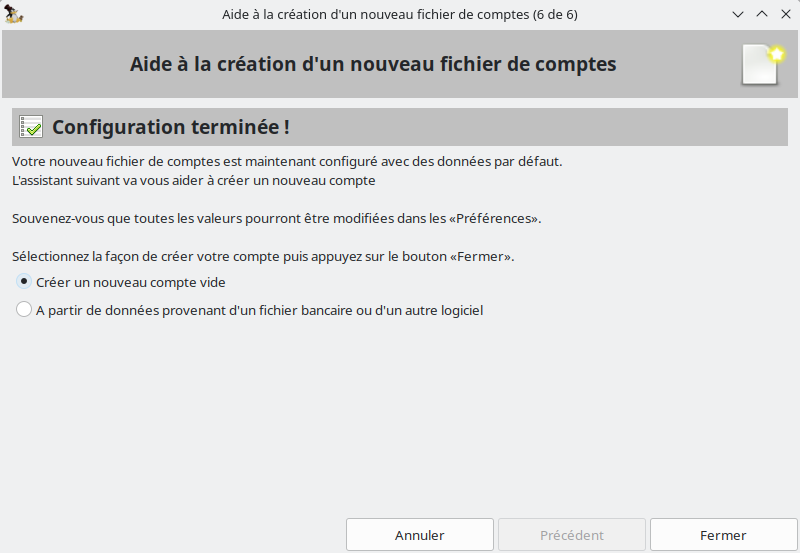
\includegraphics[scale=0.5]{image/screenshot/start_account_choice}
\end{center}
\caption{Selecting the first account}
\label{start-account-choice-img}
\end{figure}


\begin{itemize}
\item \menu{Create a new empty account}: if you check this line, then if you confirm with the \menu{Close} button, this window closes and the new account creation wizard starts. See  \vref{accounts-new}, \menu{Creating a new account},  which fully describes this procedure, then return to this page:

\item \menu{From data from a bank file or other software}: if you check this line and then confirm with the \menu{Close} button ,  this window closes and the Import Data Wizard of a file account by Grisbi starts. See the \vref{move-import-importinit} section, \menu{Importing Account Files from Another Programme into Grisbi}, which fully describes this procedure, then return to this page.
\end{itemize}
\end{enumerate}

% tiquette du paragraphe suivant, pour que les liens hypertexte dans account.tex et QIF.tex  arrivent bien dessus
\label{start-newfile-end}

\textit{\textbf{In one way or another}}, you have now created your accounts file, as well as the first account of this file.

%espace pour changement de thme
\vspacepdf{5mm}

If you want to create other accounts now, select the \menu{Edit - New Account} to create another account (see the \vref{accounts-new}, \menu{ Creating a new account} section).

%espace pour changement de thme
\vspacepdf{5mm}

Otherwise, you can start using the account you just created or the one from which you just imported the data.

% espace avant Attention ou Note : 5 mm
\vspacepdf{5mm}

\strong{Warning}: in general, it is inadvisable to have accents or spaces in the names of directories and files used by Grisbi. If so, rename them now. For example, spaces can be replaced by underscores (\underline{}).

% saut de page pour titre solidaire
\newpage


\section{Saving your accounts file\label{start-save}}

Your operations are not written as you enter them as they might be in other software; you must therefore save your account file before exiting. Do not worry, Grisbi warns you if you have not done so.

You can configure the options for saving the account file in the  \menu{ Edit - Preferences} menu, see the section \vref{setup-general-files-manage}, \menu{Managing Account Files.}.


\section{Import from other personal accounting software}

See the \vref{move-import-importinit} section to import account files from another program into Grisbi. For the moment, Grisbi supports \gls{Gnucash}, \gls{OFX}, \GLS{CSV} and \GLS{QIF} formats.


